\chapter{Application II: Semiconductor Plasma Etching}
\label{ch:etch}

Of all industrial applications of low-temperature bounded plasmas, semiconductor plasma etching is the one in which sheath physics translates most directly, and most expensively, into an engineered outcome. A modern logic or memory device is built from several hundred plasma-processing steps, many of them reactive-ion etch steps in which pattern fidelity is set by the energy and trajectory with which ions cross the sheath and strike the wafer. The sheath is the transducer that converts a bulk discharge -- characterised by $T_{\mathrm{e}}$, $n_{\mathrm{e}}$, $n_{\mathrm{i}}$ -- into a directed, quasi-monoenergetic ion beam incident on the wafer. This chapter examines how the Bohm criterion, presheath, $f_{\mathrm{i}}(v)$, and ion energy flux $\Gamma_{E}$ govern reactive ion etching (RIE), how ion energy is shaped at advanced nodes, how etch processes are monitored in production, and why in-situ, quantitative measurement of $\Gamma_E$ carries direct economic value.

\section{Reactive Ion Etching: Capacitive and Inductive Sources}

\subsection{The Reactive Ion Etching Concept}

Reactive ion etching designates dry-etch processes in which a low-pressure plasma simultaneously supplies (i) chemically reactive neutral radicals that adsorb on the wafer and form a volatile or passivating product, and (ii) energetic ions accelerated across the sheath that bombard the surface nearly normal to it. This synergy distinguishes RIE from purely chemical (isotropic) etching and purely physical sputter etching \cite{ref0536}: ion bombardment breaks surface bonds, clears passivating sidewall layers, and drives otherwise unfavourable desorption. Chemistry is set by electron-impact dissociation and ionisation in the bulk plasma; the ion-assist term is set by sheath acceleration of ions entering the presheath at the Bohm velocity,
\begin{equation}
u_{\mathrm{B}} = \sqrt{\frac{k_{\mathrm{B}} T_{\mathrm{e}}}{M}},
\label{eq:etch_bohm}
\end{equation}
with $M$ the ion mass, before crossing the sheath potential drop to the wafer. The ion flux entering the sheath is $\Gamma_{\mathrm{i}} = n_{\mathrm{s}} u_{\mathrm{B}}$, where $n_{\mathrm{s}} \approx 0.61\, n_{\mathrm{e}}$ is the sheath-edge density reduced by the presheath drop; this flux, weighted by ion energy, is the ion energy flux $\Gamma_{E}$ delivered to the wafer -- the central diagnostic quantity of this monograph.

RIE tools are almost universally RF-driven, since a DC discharge cannot be sustained against a dielectric or oxidised wafer. Two architectures dominate: capacitively coupled plasma (CCP) and inductively coupled plasma (ICP) reactors, each with its own accessible ion-energy-flux window \cite{ref0531}.

\subsection{Capacitively Coupled Plasma Reactors}

In a CCP reactor the discharge is struck between two parallel electrodes, one typically carrying the wafer, driven by an RF source from a few to several tens of \si{\mega\hertz}, with \SI{13.56}{\mega\hertz} historically dominant. The RF voltage divides between the plasma bulk and the two sheaths according to relative electrode areas and capacitances; on an asymmetric reactor with a small powered electrode and a large grounded wall, most of the applied voltage appears across the powered-electrode sheath, producing the high sheath voltages historically associated with RIE. Because the sheath is driven directly by the discharge waveform, ion density and bombardment energy are strongly coupled in single-frequency CCP: raising RF power raises both ionisation ($n_{\mathrm{e}}$, $\Gamma_{\mathrm{i}}$) and sheath voltage ($\langle E_{\mathrm{i}}\rangle$) together, limiting recipes needing high flux at fixed, moderate energy.

Dual- and multi-frequency CCP reactors break this coupling: an HF/VHF source principally sustains the plasma and sets $n_{\mathrm{e}}$, while a low-frequency source, to which ions respond quasi-statically, sets the sheath voltage swing \cite{ref0530}. RF impedance matching against the nonlinear sheath capacitance is itself nontrivial \cite{ref0531}. Chemistry is process-family specific: fluorocarbon (CF$_4$, CHF$_3$, C$_4$F$_8$) mixtures dominate dielectric (SiO$_2$, Si$_3$N$_4$) etch, chlorine/bromine chemistries dominate silicon and III--V etch, and oxygen plasmas serve resist ash and low-$k$ patterning \cite{ref0532}.

\subsection{Inductively Coupled Plasma Reactors}

An ICP reactor decouples plasma generation from wafer bias far more completely than dual-frequency CCP. Power couples inductively, via a coil separated from the plasma by a dielectric window, driving azimuthal RF currents that sustain a high-density discharge ($n_{\mathrm{e}} \sim 10^{11}$--\SI{e12}{\per\cubic\centi\meter}, one to two orders above a typical CCP) without a large sheath voltage at the source. A second, independent RF supply biases the wafer chuck, giving near-independent control of ion flux (source power) and energy (bias amplitude) \cite{ref0530}. Related variants -- electron-cyclotron-resonance sources and reactive/chemically assisted ion beam etching (RIBE/CAIBE), where a beam is extracted through a grid independently of any local sheath -- push the decoupling further \cite{ref0530}.

\subsection{Comparative Characteristics}

Table~\ref{tab:etch_ccp_icp} summarises qualitative operating characteristics of the two source families.

\begin{table}[htbp]
\centering
\caption{Qualitative comparison of capacitively and inductively coupled plasma etch sources; illustrative operating regimes, not tool specifications.}
\label{tab:etch_ccp_icp}
\begin{tabular}{@{}lll@{}}
\toprule
Characteristic & CCP (single/dual frequency) & ICP (source + bias) \\
\midrule
Typical $n_{\mathrm{e}}$ & \SI{e9}{}--\SI{e10}{\per\cubic\centi\meter} & \SI{e11}{}--\SI{e12}{\per\cubic\centi\meter} \\
Flux/energy coupling & Strongly coupled (single freq.) & Weakly coupled / independent \\
Typical sheath voltage & Hundreds of \si{\volt} & Tens to hundreds of \si{\volt} \\
Pressure regime & Higher (mTorr--Torr range) & Lower (sub-mTorr--tens mTorr) \\
Primary energy knob & RF power / LF bias amplitude & Wafer-bias generator \\
Representative use & Dielectric, polymer, blanket etch & High-aspect-ratio, damage-sensitive etch \\
\bottomrule
\end{tabular}
\end{table}

Both families remain in concurrent use, occupying complementary corners of the flux-energy-anisotropy-damage trade space of Section~\ref{sec:etch_iedf_iad}; deep silicon through-vias and Bosch-process structures, for instance, are etched almost exclusively in high-density, low-pressure ICP-type reactors.

\section{Ion Energy and Angular Distributions at the Wafer}
\label{sec:etch_iedf_iad}

\subsection{The Ion Energy Distribution Function at the Sheath Edge and Wafer}

The wafer sees not a single ion energy but a distribution, the ion energy distribution function (IEDF), obtained by propagating $f_{\mathrm{i}}(v)$ at the sheath edge through the (generally time-varying) sheath potential to the wafer. If ions cross collisionlessly and without a change of charge state, energy conservation maps the sheath-edge distribution onto the wafer-incident one through the instantaneous sheath drop $V_{\mathrm{sh}}(t)$ at arrival:
\begin{equation}
E_{\mathrm{i}} = \tfrac{1}{2} M u_{\mathrm{B}}^{2} + e\, V_{\mathrm{sh}}(t_{\mathrm{arrival}}),
\label{eq:etch_energy_map}
\end{equation}
where the first term, of order $k_{\mathrm{B}} T_{\mathrm{e}}/2$, is normally negligible compared with the second, since sheath voltages of tens to hundreds of volts vastly exceed $T_{\mathrm{e}} \sim \SI{2}{}$--\SI{5}{\electronvolt}. The ion energy flux delivered to the wafer is the first moment of this distribution,
\begin{equation}
\Gamma_{E} = \int_{0}^{\infty} E\, \Gamma_{\mathrm{i}}(E)\, \mathrm{d}E = \Gamma_{\mathrm{i}} \langle E_{\mathrm{i}} \rangle,
\label{eq:etch_gammaE}
\end{equation}
where $\Gamma_{\mathrm{i}}(E)\,\mathrm{d}E$ is the differential ion flux in $[E, E+\mathrm{d}E]$. Etch rate, selectivity, anisotropy, and damage are all functionals of $\Gamma_{\mathrm{i}}(E)$ and its angular counterpart, not of a single ``ion energy'' number -- why sheath physics rather than a scalar bias voltage is the correct level of description for RIE \cite{ref0539}.

\subsection{RF Sheath Transit Time and the Shape of the IEDF}

The IEDF shape at the wafer is controlled by the ratio of ion transit time across the sheath, $\tau_{\mathrm{i}} \sim s/u_{\mathrm{B}}$ with $s$ the time-averaged sheath thickness, to the RF period $2\pi/\omega$:

\begin{itemize}
\item \textbf{Quasi-static limit} ($\omega \tau_{\mathrm{i}} \ll 1$): ions cross quickly relative to the RF period and see an essentially fixed instantaneous voltage. Since the sheath voltage spends more time near its cycle extrema, the wafer-incident IEDF develops a bimodal (``saddle'') shape, with peaks near the minimum and maximum voltages.
\item \textbf{High-frequency limit} ($\omega \tau_{\mathrm{i}} \gg 1$): ions transit over many RF cycles and sample the time-averaged potential $\langle V_{\mathrm{sh}} \rangle$, producing a narrow, quasi-monoenergetic IEDF peaked near $e\langle V_{\mathrm{sh}} \rangle$.
\end{itemize}

This is exploited in tool design: a low-frequency bias broadens and separates the IEDF peaks (useful for sputter-clearing a passivation layer), while a high/very-high-frequency bias narrows the IEDF around a single energy, preferred when the mean, not the spread, is the control target \cite{ref0540,ref0541}. Diagnostic development has targeted this bimodal-to-monoenergetic transition as the observable a sensor must resolve. Figure~\ref{fig:etch_iedf} sketches the qualitative transition with an illustrative sum-of-Gaussians model; it is not measured or simulated data.

\begin{figure}[htbp]
\centering
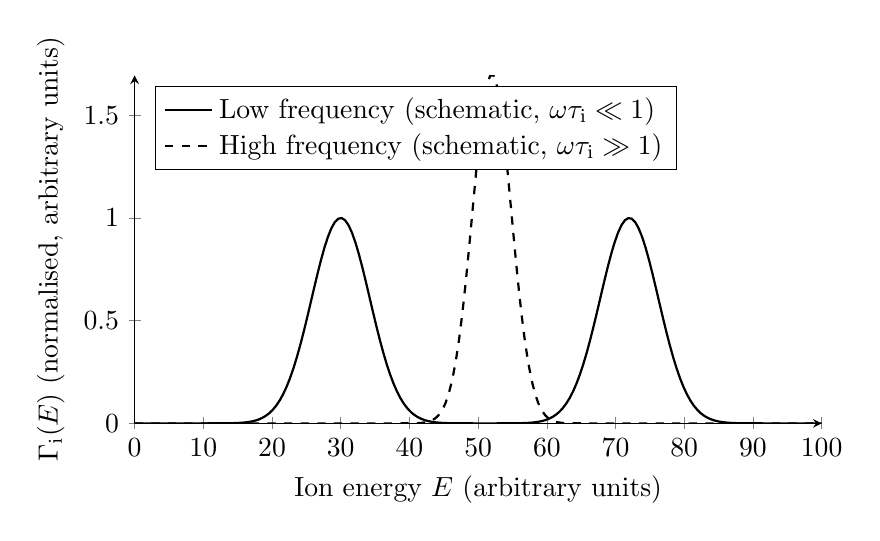
\begin{tikzpicture}
\begin{axis}[
 width=0.85\linewidth, height=6cm,
 xlabel={Ion energy $E$ (arbitrary units)},
 ylabel={$\Gamma_{\mathrm i}(E)$ (normalised, arbitrary units)},
 domain=0:100, samples=200,
 no markers, axis lines=left,
 legend pos=north west, legend cell align=left,
 ymin=0
]
\addplot[thick, solid, black]
 {exp(-((x-30)/6)^2) + exp(-((x-72)/6)^2)};
\addlegendentry{Low frequency (schematic, $\omega\tau_{\mathrm i}\ll1$)}
\addplot[thick, dashed, black]
 {1.7*exp(-((x-52)/4)^2)};
\addlegendentry{High frequency (schematic, $\omega\tau_{\mathrm i}\gg1$)}
\end{axis}
\end{tikzpicture}
\caption{Schematic ion energy distribution functions at the wafer for the low-frequency (bimodal) and high-frequency (narrow, quasi-monoenergetic) sheath-transit regimes, from an arbitrary sum-of-Gaussians expression; not measured or simulated data.}
\label{fig:etch_iedf}
\end{figure}

The sheath voltage, and hence the IEDF's position on the energy axis, is set by the Child--Langmuir space-charge law relating sheath current density $J$, applied voltage $V$, and time-averaged sheath thickness $s$,
\begin{equation}
J = \frac{4}{9}\, \varepsilon_{0} \sqrt{\frac{2e}{M}}\; \frac{V^{3/2}}{s^{2}},
\label{eq:etch_cl}
\end{equation}
so that, for fixed ion flux $J/e = \Gamma_{\mathrm{i}}$, sheath thickness must expand as $s \propto V^{3/4}$ as bias voltage rises -- the sheath accelerates ions more strongly and grows thicker together. Figure~\ref{fig:etch_cl} shows the corresponding Child--Langmuir potential profile, again analytic rather than measured.

\begin{figure}[htbp]
\centering
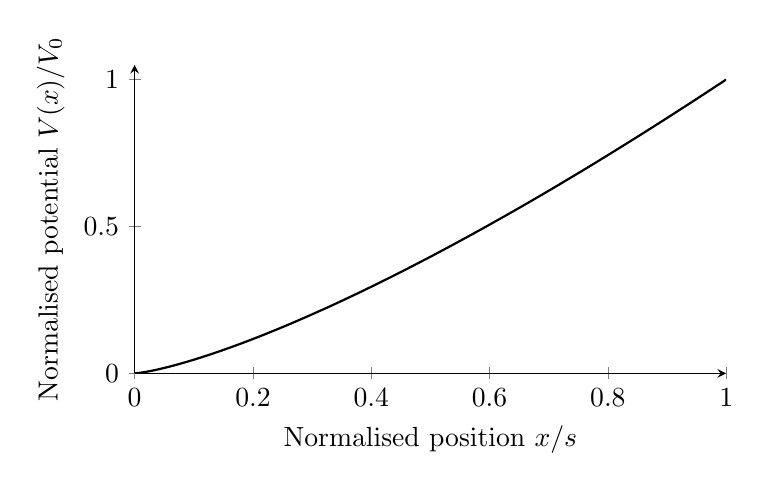
\begin{tikzpicture}
\begin{axis}[
 width=0.75\linewidth, height=5.5cm,
 xlabel={Normalised position $x/s$},
 ylabel={Normalised potential $V(x)/V_{0}$},
 domain=0:1, samples=100,
 no markers, axis lines=left,
 ymin=0, ymax=1.05
]
\addplot[thick, black] {x^(4/3)};
\end{axis}
\end{tikzpicture}
\caption{Schematic Child--Langmuir potential profile $V(x)/V_{0} = (x/s)^{4/3}$ across a collisionless, space-charge-limited planar sheath; illustrative of the functional form only.}
\label{fig:etch_cl}
\end{figure}

\subsection{Ion Angular Distributions and the Origin of Anisotropy}

Anisotropic (directional) etching -- etching straight down through a mask opening without appreciable lateral undercut -- is the capability that distinguishes RIE from wet or purely chemical dry etching, and derives directly from the ion angular distribution function (IADF) delivered by the sheath. Because the sheath field is, to good approximation, one-dimensional and normal to the wafer, ions accelerated across a thin, collisionless sheath arrive clustered near the surface normal; any transverse velocity, of order $\sqrt{k_{\mathrm{B}}T_{\mathrm{i}}/M}$, divides by the much larger normal velocity, so the IADF narrows as sheath voltage increases. Two effects broaden it: collisions with neutrals once $s$ is not small compared with the ion mean free path, and RF modulation of the sheath edge, introducing a time-dependent transverse kick correlated with the transit-time effects above. Anisotropy is a quantitative, energy- and pressure-dependent outcome, summarised by
\begin{equation}
A = 1 - \frac{\mathrm{ER}_{\mathrm{lateral}}}{\mathrm{ER}_{\mathrm{vertical}}},
\label{eq:etch_aniso}
\end{equation}
with $A \to 1$ for perfectly anisotropic and $A \to 0$ for isotropic etching, where $\mathrm{ER}_{\mathrm{vertical}}$ and $\mathrm{ER}_{\mathrm{lateral}}$ are the etch rates normal to, and parallel to, the sidewall. High-aspect-ratio processes such as deep RIE of silicon through-vias and MEMS structures depend on maintaining a narrow IADF and self-passivating sidewall chemistry across the full feature depth; their principal failure modes -- scalloping, bowing, and aspect-ratio-dependent etch-rate lag (``RIE lag'') -- are fingerprints of angular and energy broadening compounded with neutral-transport limits deep in a trench. Crystallographic and hard-mask-dependent variants recur across diamond, silicon carbide, graphene, and III--V compound semiconductors.

\subsection{Etch Selectivity as an Energy-Threshold Phenomenon}

Selectivity, for two materials A (the film etched) and B (a stop layer, sidewall, or mask), is the ratio of their etch rates,
\begin{equation}
S_{\mathrm{A/B}} = \frac{\mathrm{ER}_{\mathrm{A}}}{\mathrm{ER}_{\mathrm{B}}},
\label{eq:etch_select}
\end{equation}
controlled by the same IEDF, but through an energy threshold. Ion-assisted etch yield typically follows a Sigmund-type threshold law
\begin{equation}
Y(E) =
\begin{cases}
0, & E \le E_{\mathrm{th}} \\
A_{\mathrm{Y}} \left( \sqrt{E} - \sqrt{E_{\mathrm{th}}} \right), & E > E_{\mathrm{th}}
\end{cases}
\label{eq:etch_yield}
\end{equation}
where $E_{\mathrm{th}}$ is a material- and chemistry-dependent threshold below which no ion-assisted removal occurs, and $A_{\mathrm{Y}}$ a normalisation constant. Because $E_{\mathrm{th}}$ differs between film and stop layer, a window can in principle be found with $\langle E_{\mathrm{i}} \rangle$ above $E_{\mathrm{th,A}}$ but below $E_{\mathrm{th,B}}$, giving effectively infinite selectivity in the ideal, single-energy limit. In practice the finite IEDF width erodes this: any high-energy tail above $E_{\mathrm{th,B}}$ erodes the stop layer directly, so achievable selectivity is set by the fraction of the IEDF above the more restrictive threshold. Selectivity-limited processes -- gate-oxide overetch stopping on channel silicon, or metal-gate etch stopping on a high-$\kappa$ dielectric -- are therefore controlled through IEDF tailoring rather than mean bias voltage \cite{ref0539,ref0541}. Demonstrations for hydrogen-ion-driven RIE of tin films and oxygen-plasma etching of polymer resists \cite{ref0532} are consistent with this threshold-type law.

\subsection{Plasma-Induced Damage}

The same ion bombardment enabling anisotropic pattern transfer is the principal source of plasma-induced damage, coupled through the same IEDF rather than independently tunable. Damage falls into three categories: physical lattice damage (point defects, amorphisation, implantation) scaling with the high-energy tail and ion mass; charging damage, where a fluctuating sheath potential drives charge accumulation that ruptures thin gate dielectrics; and chemical/compositional damage, where bombardment with reactive species alters stoichiometry or dopant profile. All three worsen, for fixed mean energy, when the IEDF has a broad or high-energy tail -- exactly what quasi-static operation or uncontrolled RF harmonic content produces. Sub-5-nm processes (Section~\ref{sec:etch_advanced}) therefore emphasise synthesising narrow, precisely bounded IEDFs rather than simply lowering mean bias voltage \cite{ref0539,ref0541}.

\section{Ion Energy Control at Advanced (Sub-5 nm) Nodes}
\label{sec:etch_advanced}

\subsection{Why Ion Energy Control Becomes Critical Below 5 nm}

As device pitch shrinks into the sub-5-nm regime -- fin and nanosheet FETs, self-aligned multiple patterning, atomic-scale gate stacks -- the etch budget for imprecision in ion energy collapses. Several node-scaling effects compound to make ion-energy-flux control a first-order parameter:

\begin{itemize}
\item \textbf{Shrinking selectivity margins.} As gate dielectrics, spacers, and liners scale to a few nanometres, the overetch budget before the stop layer is compromised shrinks, so even a modest high-energy tail becomes yield-limiting.
\item \textbf{Aspect-ratio inflation.} Area scaling at roughly constant film thickness drives aspect ratios upward, narrowing angular tolerance and sensitivity to IADF broadening.
\item \textbf{Damage-sensitive materials.} High-mobility channel materials, ultra-thin bodies, and high-$\kappa$/metal-gate stacks are intrinsically more sensitive to lattice and charging damage per incident ion.
\item \textbf{Line-edge roughness and stochastics.} At sub-5-nm dimensions, discreteness of individual ion impacts and statistical fluctuation of local flux become comparable to feature size, so the full IEDF shape, not just its mean, determines edge-placement error.
\end{itemize}

These pressures have driven a shift in tool architecture away from simple bias-voltage control toward direct synthesis of a target IEDF shape \cite{ref0539,ref0540,ref0541}.

\subsection{Tailored-Waveform and Electrical Asymmetry Techniques}

The most direct route to a narrow, precisely positioned IEDF is a custom, non-sinusoidal voltage waveform on the wafer electrode. Summing multiple harmonics with controlled relative phase and amplitude sculpts the sheath voltage to dwell near a single target voltage for an extended fraction of each cycle, which, combined with transit-time filtering, compresses the wafer-incident IEDF toward a narrow, single-peaked distribution rather than a broader bimodal one. This family of techniques, known as tailored ion energy distributions or the electrical asymmetry effect, allows mean ion energy and IEDF width to be set as separate process variables \cite{ref0541}. Magnetic-field-assisted sheath tailoring is a complementary route, modifying ion trajectories at non-planar features. Dual-RF excitation is the architectural precursor to full waveform tailoring and remains in widespread use where arbitrary-waveform generators are not required.

\subsection{Pulsed-Plasma and Synchronous Pulsed-Bias Schemes}

A second control axis is time-domain pulsing, in which source power, bias power, or both are switched between set points on a timescale slow compared with the RF period but comparable to or faster than plasma-chemistry relaxation. Synchronous pulsing divides an etch cycle into sub-steps -- a chemistry-dominated deposition/passivation sub-step with bias suppressed, followed by an ion-dominated activation sub-step with bias raised -- so the ion energy flux delivered per cycle is tuned more finely, with far less unwanted high-energy tail, than with continuous-wave bias alone. Repetitive pulsed-power schemes extend this by exploiting the afterglow between pulses (where $T_{\mathrm{e}}$ collapses while $n_{\mathrm{e}}$ decays more slowly) to deliver a naturally narrow, low-energy ion population for damage-sensitive steps. Pulsed and pulsed-DC bias schemes have been directly characterised by IEDF measurement, confirming the pulse envelope reproducibly reshapes the energy distribution \cite{ref0540}.

\subsection{Atomic Layer Etching as the Limiting Case of Energy Control}

Atomic layer etching (ALE) is the extreme, self-limiting endpoint of ion energy control: the cycle splits into a chemical modification sub-step (a low-energy, near-thermal exposure converting a fixed number of surface atomic layers into a weakly bound species) and a removal sub-step in which a low-energy, narrow-IEDF ion pulse -- mean energy just above the removal threshold of the modified layer and just below that of the underlying material -- desorbs exactly the modified layer and no more. Because removal relies on the gap between two closely spaced thresholds, ALE is far more sensitive to IEDF width and tail content than continuous RIE: a tail extending even modestly above the substrate threshold erodes the self-limiting character that makes it valuable. Reliable, sub-nanometre-per-cycle removal therefore depends directly on the tailored-waveform and pulsed-bias techniques above \cite{ref0539,ref0541}.

\section{Process Monitoring, Endpoint Detection and Control}

\subsection{Optical Emission Spectroscopy Endpoint Detection}

The most widely deployed real-time monitoring technique in production RIE is optical emission spectroscopy (OES) endpoint detection, in which the intensity of a characteristic emission line -- typically from an etch-product species (e.g.\ SiF during silicon or SiO$_2$ etch) or a depleted reactant -- is tracked through an etch step. When the film clears and the underlying, chemically different stop layer is exposed, the plasma chemistry shifts abruptly, producing a step change used to trigger step termination or an overetch sub-recipe. OES is attractive because it is non-invasive and responds directly to a chemical signature of the process. Its principal limitation is that it monitors the chemical, not the physical (ion-energy), half of RIE: an OES trace can detect that a film has cleared but cannot tell whether the delivered ion energy flux was within specification -- an acceptable endpoint trace can still coexist with an out-of-specification profile, selectivity, or damage level.

\subsection{Electrical and Particle-Based Diagnostics}

Because OES leaves the ion-energy-flux dimension unmonitored, production and development tools are commonly instrumented with complementary electrical and particle diagnostics. Laser-induced fluorescence provides spatially resolved measurements of reactive species and ion velocity information OES cannot. Retarding-field energy analysers (RFEAs), typically embedded in or substituted for a witness wafer, provide a direct, energy-resolved measurement of the IEDF and IADF at a wafer-plane location and are the standard tool for characterising the waveforms of Section~\ref{sec:etch_advanced} \cite{ref0548,ref0556}. Broader diagnostic suites -- Langmuir-probe-family probes, ion/neutral mass spectrometry, and closed-loop-control sensors -- are reviewed in the process-diagnostics literature \cite{ref0548,ref0553,ref0556}. Plasma immersion ion implantation tools, using the wafer sheath itself in a pulsed high-voltage configuration, are an especially direct case where delivered ion energy flux is the entire process variable of interest.

\subsection{Model-Based and Virtual-Metrology Control}

Production fabs increasingly supplement direct sensor readings with model-based and virtual-metrology approaches, in which a physical or empirical model of the sheath and reactor -- informed by chamber telemetry such as RF forward/reflected power, matching-network tap positions, gas flows, and pressure -- infers the IEDF or ion energy flux at the wafer without a dedicated in-situ sensor on every run. Such models are calibrated periodically against direct RFEA or witness-wafer measurements, then used between calibrations to flag drift in the inferred $\Gamma_{E}$. This matters because RFEA-type sensors are frequently incompatible with continuous, wafer-by-wafer production, so the diagnostics community has pursued sensor concepts -- wafer-embedded and non-invasive real-time architectures -- explicitly designed for production compatibility \cite{ref0548,ref0553}.

\section{Value of In-Situ Ion-Energy-Flux Measurement for Yield}

\subsection{Cost of Process Excursions in Advanced Fabrication}

An advanced-node fabrication line represents enormous accumulated capital and cycle-time investment by the time a wafer reaches any individual etch chamber: hundreds of prior process steps, each with its own yield-loss probability, have already been applied. An etch excursion -- an undetected drift of the delivered ion energy flux, from electrode erosion, RF-match ageing, or gradual contamination -- that shifts the IEDF mean, broadens it, or populates its high-energy tail can simultaneously degrade critical-dimension control, erode selectivity margins, and elevate damage across every wafer processed before the next scheduled maintenance event catches the drift. Because OES endpoint detection is largely blind to this class of excursion, the interval between onset and detection can span many lots, and the yield impact scales with wafers processed before detection -- making detection latency itself, not merely the root-cause fix, a first-order economic quantity.

\subsection{Ion-Energy-Flux Metrology as a Yield Lever}

A quantitative, continuously available measurement of $\Gamma_{E}$ at, or representative of, the wafer plane closes exactly this monitoring gap. Where OES answers ``has the correct film been removed,'' and post-etch metrology answers ``was the correct feature produced,'' an ion-energy-flux sensor answers the physically upstream question -- ``was the sheath delivering the ion population the recipe assumed'' -- at the timescale of the process step itself. This matters because $\Gamma_{E}$ is a leading indicator: a drift in the sheath-delivered ion energy flux precedes, and causally produces, downstream anisotropy, selectivity, and damage excursions rather than merely correlating with them. Diagnostic development aimed at real-time, non-invasive IEDF monitoring and in-line wafer-type sensors has been motivated directly by this leading-indicator argument \cite{ref0539,ref0541}. The same argument extends to related processes such as plasma immersion ion implantation doping; diagnostics reviews treat ion-energy-flux sensing as a general-purpose capability across this family of processes \cite{ref0553,ref0556}.

\subsection{Integration Path into Production Tools}

Translating an ion-energy-flux sensor from a laboratory diagnostic into a production-compatible capability requires constraints largely orthogonal to raw measurement fidelity: it must not consume a wafer slot on every run, must survive the chemically aggressive environment over an extended service interval, must report on a timescale compatible with real-time recipe feedback, and must integrate with existing fab data infrastructure (SPC charts, fault-detection-and-classification systems). Wafer-embedded sensor designs, RFEA-derived architectures adapted for durability, and model-based virtual metrology each represent a different point on this trade-off, and the diagnostics literature has pursued all three routes in parallel \cite{ref0548,ref0553,ref0556}. The common thread is the same sheath physics developed throughout this monograph: such a sensor is, at its core, an instrument for measuring $\Gamma_{E} = \int E\, \Gamma_{\mathrm{i}}(E)\, \mathrm{d}E$ at a surface, and every design choice is a direct response to the shape and stability requirements the sheath places on $\Gamma_{\mathrm{i}}(E)$.

\section{Summary}

Reactive ion etching converts the sheath physics developed earlier in this monograph into the dominant pattern-transfer technology of the semiconductor industry: capacitively and inductively coupled sources generate the bulk plasma and, through single-, dual-, or multi-frequency bias schemes, set the sheath voltage that determines ion energy delivered to the wafer. The wafer-incident ion population is fully characterised only by its joint energy and angular distribution, shaped by ion transit time relative to the RF period and by collisional broadening; anisotropy, selectivity, and plasma-induced damage are all functionals of this same distribution rather than independently tunable outcomes. At sub-5-nm nodes, shrinking overetch and damage budgets have driven a shift from simple bias-voltage control toward direct synthesis of a target IEDF shape through tailored waveforms, electrical asymmetry techniques, synchronous pulsing, and, in its most extreme form, atomic layer etching. Production monitoring today rests primarily on OES endpoint detection, sensitive to etch chemistry but blind to the ion-energy-flux dimension, leaving a diagnostic gap between the upstream cause of many excursions and their eventual downstream detection. Closing that gap with a quantitative, in-situ, production-compatible measurement of $\Gamma_{E}$ functions as a leading-indicator yield lever, and the path to such a sensor is, at its foundation, an application of the same Bohm-criterion, presheath, and sheath-transport physics that has organised this monograph.
